%%% Local Variables:
%%% mode: latex
%%% TeX-master: "../report"
%%% End:

\subsection{Definition of terms}
\begin{description}
\item[Compiler] \hfill \\
  A program that translates (potentially high-level) program code into
  another language. Common targets are assembly languages for either
  hardware CPUs or abstract machines. Examples include
  \texttt{gcc}\cite{NEEDED}, \texttt{javac}\cite{NEEDED} and
  \texttt{ghc}\cite{NEEDED}.

\item[Object-Orientation] \hfill \\
  Foo bar

\item[Intermediate Language (or Intermediate Representation)] \hfill \\

\end{description}


% \subsection{\thename{} Specification}
\label{sec:spec}
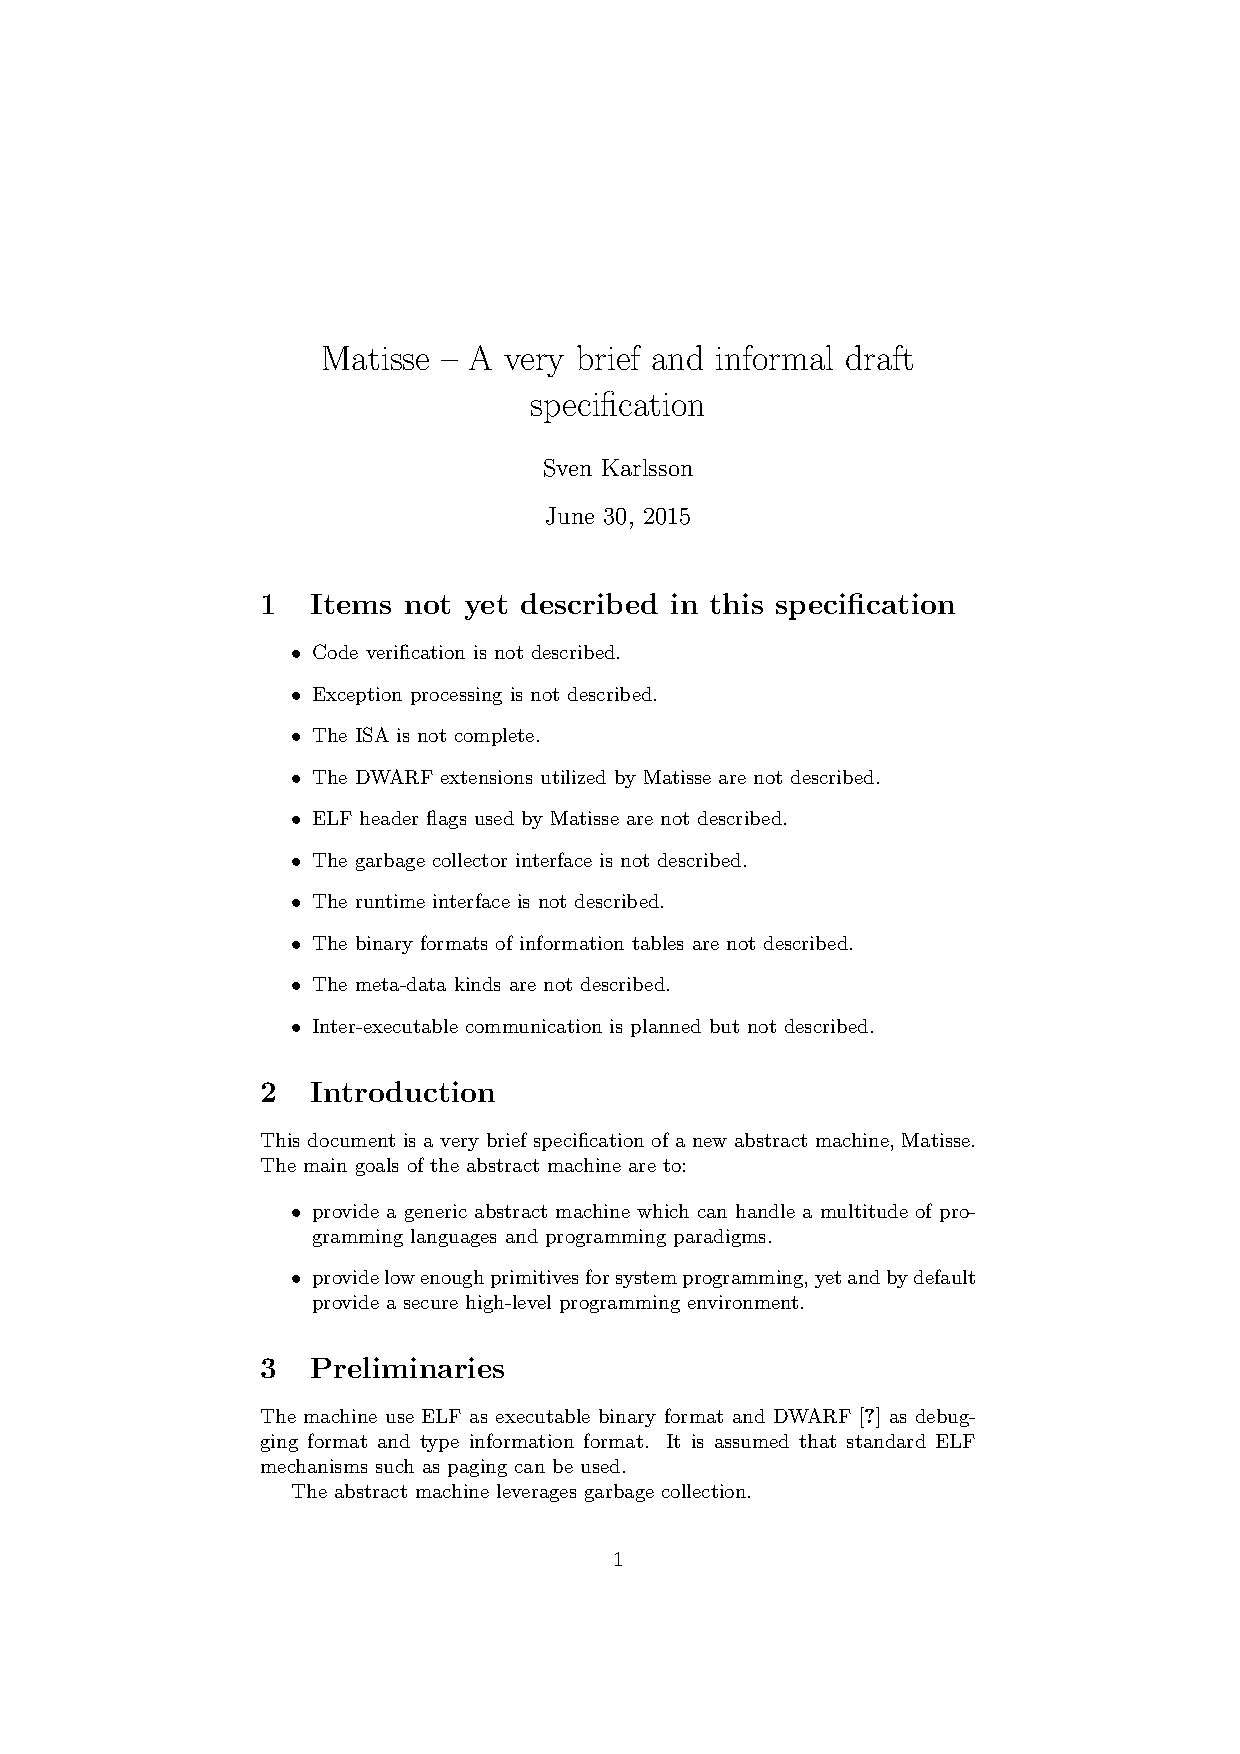
\includepdf[pages=-]{lib/spec.pdf}
